% Source of the figure chain-link-types.pdf (the chain links of one variable).
% Compile with pdfLaTeX; the PDF is included in the manuscript at its natural size.
\documentclass[tikz,border=1pt]{standalone}
\usepackage[T1]{fontenc}
\usepackage{stix}
\pdfinfoomitdate=1 \pdftrailerid{} \pdfsuppressptexinfo=-1
\definecolor{threadred}{RGB}{200,40,40}
\begin{document}
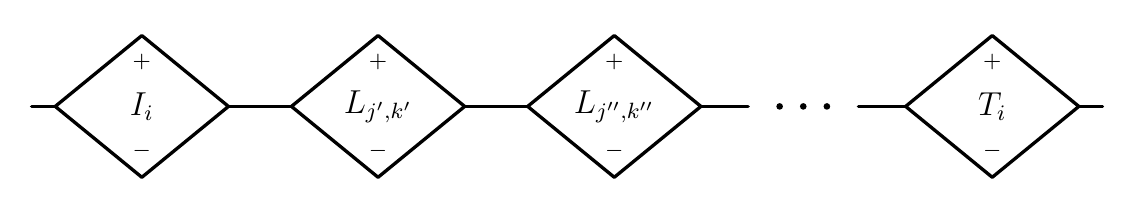
\begin{tikzpicture}[x=1cm, y=1cm,
    chain/.style={line width=1.2pt, line cap=round, line join=round},
    thread/.style={line width=0.8pt, line cap=round},
    crossing/.style={line width=2.6pt, line cap=butt},
    lead/.style={thread, densely dashed}]
  % A chain link: #1 = x-coordinate of its center, #2 = its name.
  % The upper path is the positive path, the lower path the negative path.
  \newcommand{\chainlink}[2]{%
    \draw[chain] (#1-1.1,0) -- (#1,0.9) -- (#1+1.1,0) -- (#1,-0.9) -- cycle;
    \node at (#1,0) {\large #2};
    \node at (#1,0.56) {\footnotesize $+$};
    \node at (#1,-0.56) {\footnotesize $-$};}

  \useasboundingbox (0.15,-1.0) rectangle (13.85,1.0);
  \chainlink{1.6}{$I_i$}
  \chainlink{4.6}{$L_{j',k'}$}
  \chainlink{7.6}{$L_{j'',k''}$}
  \chainlink{12.4}{$T_i$}
  \draw[chain] (0.2,0) -- (0.5,0)  (2.7,0) -- (3.5,0)  (5.7,0) -- (6.5,0)  (8.7,0) -- (9.3,0)
               (10.7,0) -- (11.3,0)  (13.5,0) -- (13.8,0);
  \foreach \x in {9.7,10.0,10.3} \fill (\x,0) circle[radius=1.2pt];
\end{tikzpicture}
\end{document}
